\documentclass{standalone}
\usepackage{tikz}
\usetikzlibrary{patterns, positioning}
\usepackage[sfdefault]{ClearSans} %% option 'sfdefault' activates Clear Sans as the default text font
\usepackage[T1]{fontenc}

\begin{document}
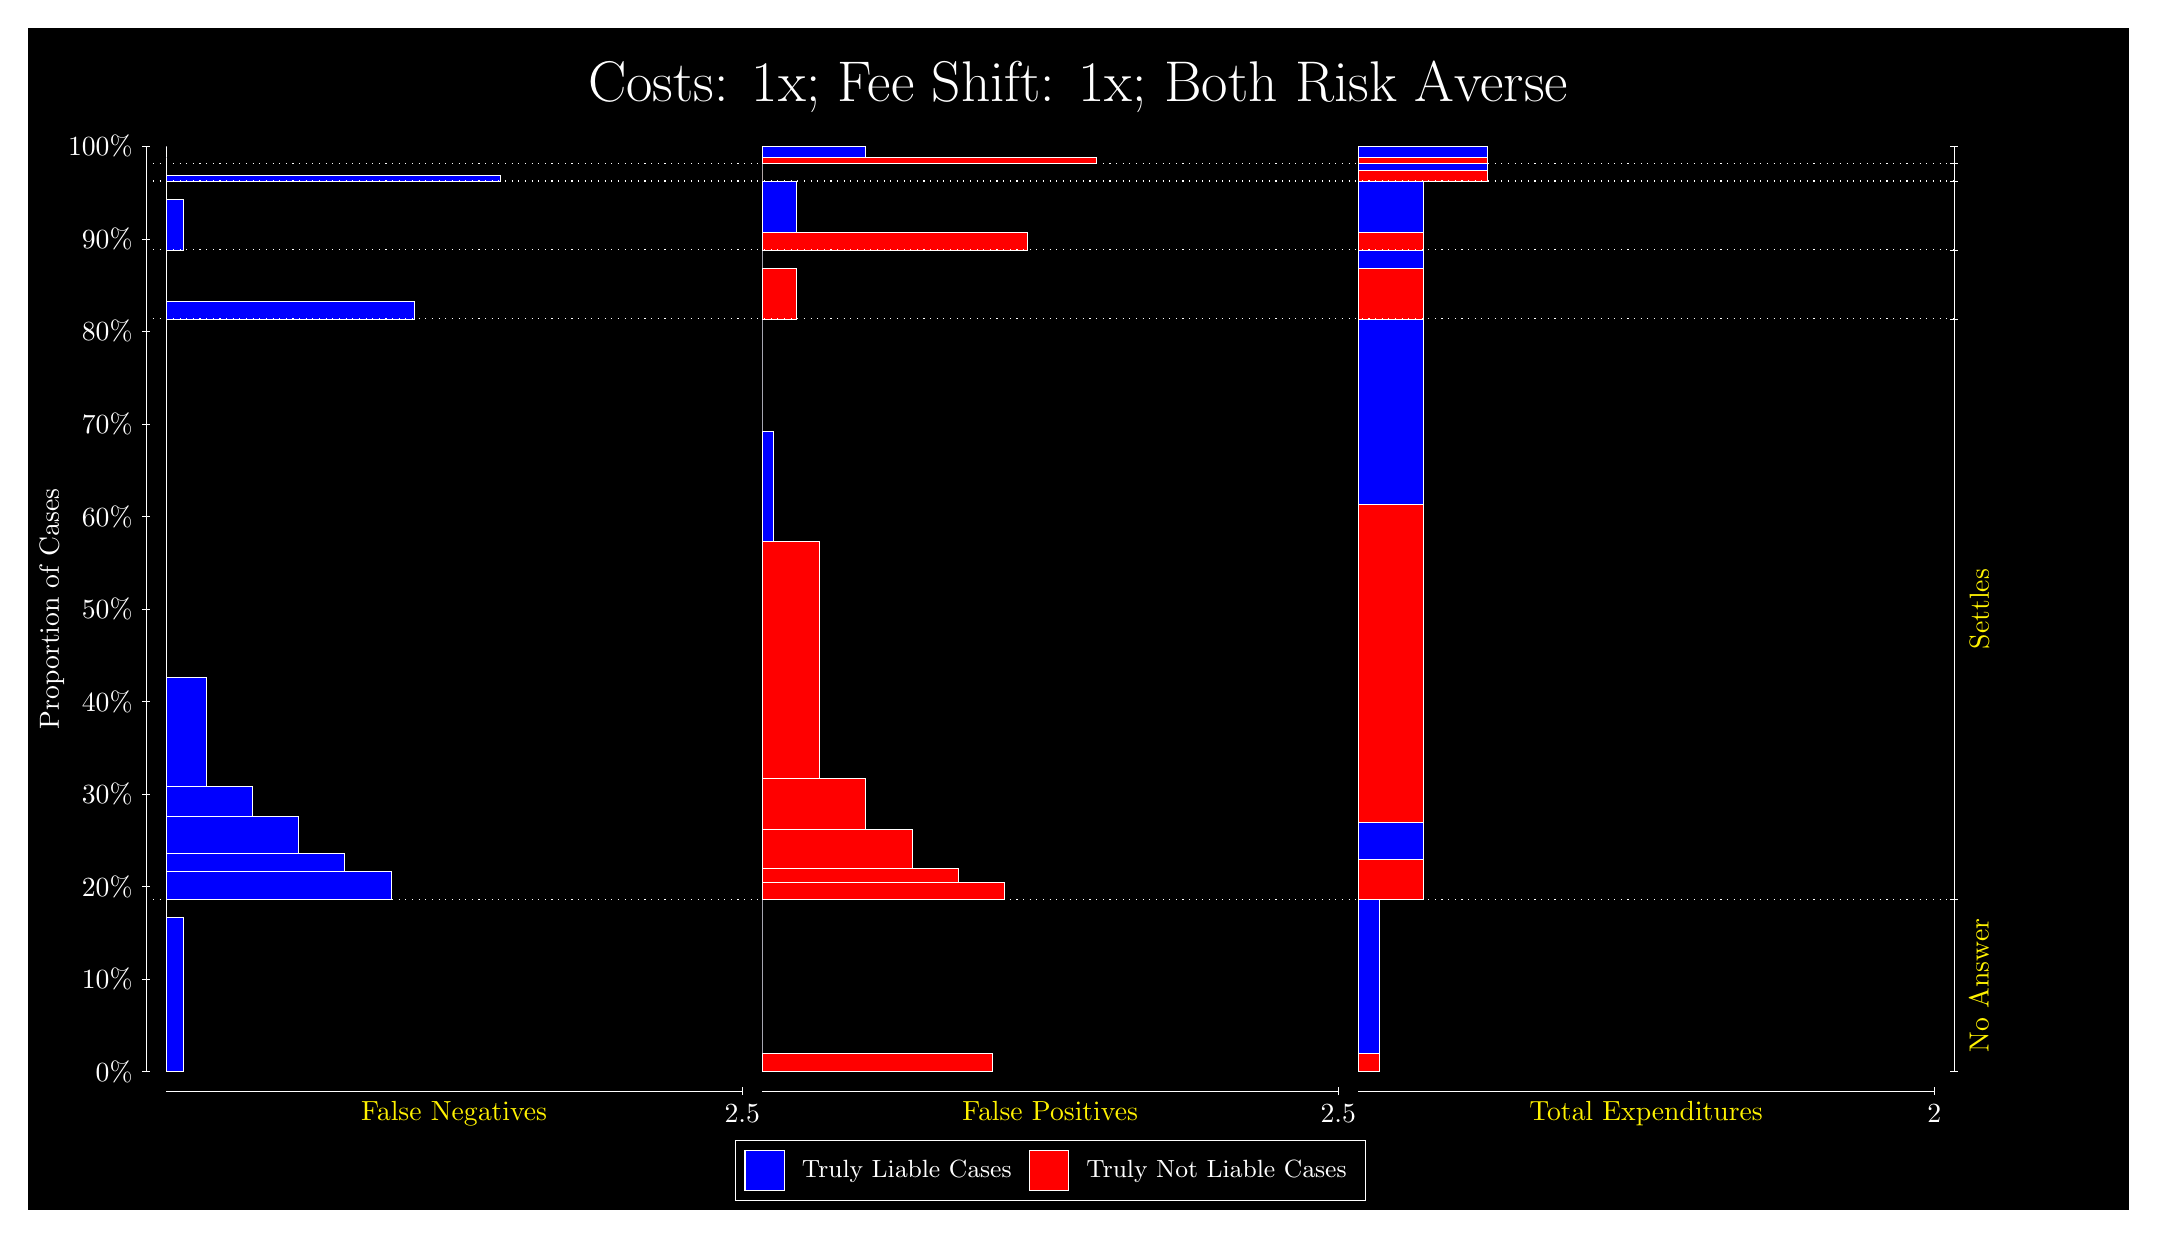
\begin{tikzpicture}
\draw[fill=black] (0,0) rectangle (26.667,15);
\draw[text=white] (0,13.5) rectangle (26.667,15) node[midway] {\huge Costs: 1x; Fee Shift: 1x; Both Risk Averse};
\draw[white, very thin] (1.5,1.75) -- (1.5,13.5);
\node[rotate=90, text=white, anchor=center] at (0.3, 7.625) {Proportion of Cases};
\draw[white, very thin] (1.45,1.75) -- (1.55,1.75);
\node[text=white, anchor=east] at (1.45, 1.75) {0\%};
\draw[white, very thin] (1.45,2.925) -- (1.55,2.925);
\node[text=white, anchor=east] at (1.45, 2.925) {10\%};
\draw[white, very thin] (1.45,4.1) -- (1.55,4.1);
\node[text=white, anchor=east] at (1.45, 4.1) {20\%};
\draw[white, very thin] (1.45,5.275) -- (1.55,5.275);
\node[text=white, anchor=east] at (1.45, 5.275) {30\%};
\draw[white, very thin] (1.45,6.45) -- (1.55,6.45);
\node[text=white, anchor=east] at (1.45, 6.45) {40\%};
\draw[white, very thin] (1.45,7.625) -- (1.55,7.625);
\node[text=white, anchor=east] at (1.45, 7.625) {50\%};
\draw[white, very thin] (1.45,8.8) -- (1.55,8.8);
\node[text=white, anchor=east] at (1.45, 8.8) {60\%};
\draw[white, very thin] (1.45,9.975) -- (1.55,9.975);
\node[text=white, anchor=east] at (1.45, 9.975) {70\%};
\draw[white, very thin] (1.45,11.15) -- (1.55,11.15);
\node[text=white, anchor=east] at (1.45, 11.15) {80\%};
\draw[white, very thin] (1.45,12.325) -- (1.55,12.325);
\node[text=white, anchor=east] at (1.45, 12.325) {90\%};
\draw[white, very thin] (1.45,13.5) -- (1.55,13.5);
\node[text=white, anchor=east] at (1.45, 13.5) {100\%};

\draw[white, very thin] (24.457,1.75) -- (24.457,13.5);
\draw[white, very thin] (24.407,1.75) -- (24.507,1.75);
\node[anchor=west] at (24.407, 1.75) {};
\draw[white, very thin] (24.407,3.9362) -- (24.507,3.9362);
\node[anchor=west] at (24.407, 3.9362) {};
\draw[white, very thin] (24.407,11.309) -- (24.507,11.309);
\node[anchor=west] at (24.407, 11.309) {};
\draw[white, very thin] (24.407,12.184) -- (24.507,12.184);
\node[anchor=west] at (24.407, 12.184) {};
\draw[white, very thin] (24.407,13.059) -- (24.507,13.059);
\node[anchor=west] at (24.407, 13.059) {};
\draw[white, very thin] (24.407,13.28) -- (24.507,13.28);
\node[anchor=west] at (24.407, 13.28) {};
\draw[white, very thin] (24.407,13.5) -- (24.507,13.5);
\node[anchor=west] at (24.407, 13.5) {};

\draw[white, very thin, fill=blue] (1.75,1.75) rectangle (1.9696,3.7062);
\draw[white, very thin, fill=red] (1.75,3.7062) rectangle (1.75,3.9362);
\draw[white, very thin, fill=blue] (1.75,3.9362) rectangle (4.6044,4.2944);
\draw[white, very thin, fill=blue] (1.75,4.2944) rectangle (4.0188,4.5216);
\draw[white, very thin, fill=blue] (1.75,4.5216) rectangle (3.4333,4.9932);
\draw[white, very thin, fill=blue] (1.75,4.9932) rectangle (2.8478,5.3685);
\draw[white, very thin, fill=blue] (1.75,5.3685) rectangle (2.2623,6.7596);
\draw[white, very thin, fill=red] (1.75,6.7596) rectangle (1.75,11.309);
\draw[white, very thin, fill=blue] (1.75,11.309) rectangle (4.8971,11.536);
\draw[white, very thin, fill=red] (1.75,11.536) rectangle (1.75,12.184);
\draw[white, very thin, fill=blue] (1.75,12.184) rectangle (1.9696,12.832);
\draw[white, very thin, fill=red] (1.75,12.832) rectangle (1.75,13.059);
\draw[white, very thin, fill=blue] (1.75,13.059) rectangle (5.9949,13.137);
\draw[white, very thin, fill=red] (1.75,13.137) rectangle (1.75,13.28);
\draw[white, very thin, fill=red] (1.75,13.28) rectangle (1.75,13.357);
\draw[white, very thin, fill=blue] (1.75,13.357) rectangle (1.75,13.5);
\draw[white, very thin, fill=red] (9.3189,1.75) rectangle (12.246,1.98);
\draw[white, very thin, fill=blue] (9.3189,1.98) rectangle (9.3189,3.9362);
\draw[white, very thin, fill=red] (9.3189,3.9362) rectangle (12.393,4.1563);
\draw[white, very thin, fill=red] (9.3189,4.1563) rectangle (11.807,4.3263);
\draw[white, very thin, fill=red] (9.3189,4.3263) rectangle (11.222,4.8303);
\draw[white, very thin, fill=red] (9.3189,4.8303) rectangle (10.636,5.478);
\draw[white, very thin, fill=red] (9.3189,5.478) rectangle (10.051,8.4859);
\draw[white, very thin, fill=blue] (9.3189,8.4859) rectangle (9.4652,9.8769);
\draw[white, very thin, fill=blue] (9.3189,9.8769) rectangle (9.3189,11.309);
\draw[white, very thin, fill=red] (9.3189,11.309) rectangle (9.758,11.957);
\draw[white, very thin, fill=blue] (9.3189,11.957) rectangle (9.3189,12.184);
\draw[white, very thin, fill=red] (9.3189,12.184) rectangle (12.686,12.411);
\draw[white, very thin, fill=blue] (9.3189,12.411) rectangle (9.758,13.059);
\draw[white, very thin, fill=red] (9.3189,13.059) rectangle (9.3189,13.202);
\draw[white, very thin, fill=blue] (9.3189,13.202) rectangle (9.3189,13.28);
\draw[white, very thin, fill=red] (9.3189,13.28) rectangle (13.564,13.357);
\draw[white, very thin, fill=blue] (9.3189,13.357) rectangle (10.636,13.5);
\draw[white, very thin, fill=red] (16.888,1.75) rectangle (17.162,1.98);
\draw[white, very thin, fill=blue] (16.888,1.98) rectangle (17.162,3.9362);
\draw[white, very thin, fill=red] (16.888,3.9362) rectangle (17.711,4.4402);
\draw[white, very thin, fill=blue] (16.888,4.4402) rectangle (17.711,4.9118);
\draw[white, very thin, fill=red] (16.888,4.9118) rectangle (17.711,8.9575);
\draw[white, very thin, fill=blue] (16.888,8.9575) rectangle (17.711,11.309);
\draw[white, very thin, fill=red] (16.888,11.309) rectangle (17.711,11.957);
\draw[white, very thin, fill=blue] (16.888,11.957) rectangle (17.711,12.184);
\draw[white, very thin, fill=red] (16.888,12.184) rectangle (17.711,12.411);
\draw[white, very thin, fill=blue] (16.888,12.411) rectangle (17.711,13.059);
\draw[white, very thin, fill=red] (16.888,13.059) rectangle (18.534,13.202);
\draw[white, very thin, fill=blue] (16.888,13.202) rectangle (18.534,13.28);
\draw[white, very thin, fill=red] (16.888,13.28) rectangle (18.534,13.357);
\draw[white, very thin, fill=blue] (16.888,13.357) rectangle (18.534,13.5);
\draw[white, dotted] (1.5,3.9362) -- (24.457,3.9362);
\draw[white, dotted] (1.5,11.309) -- (24.457,11.309);
\draw[white, dotted] (1.5,12.184) -- (24.457,12.184);
\draw[white, dotted] (1.5,13.059) -- (24.457,13.059);
\draw[white, dotted] (1.5,13.28) -- (24.457,13.28);
\draw[white, very thin] (1.75,1.5) -- (9.0689,1.5);
\node[text=yellow, anchor=north] at (5.4094, 1.5) {False Negatives};
\draw[white, very thin] (9.0689,1.45) -- (9.0689,1.55);
\node[text=white, anchor=north] at (9.0689, 1.45) {2.5};

\draw[white, very thin] (9.3189,1.5) -- (16.638,1.5);
\node[text=yellow, anchor=north] at (12.978, 1.5) {False Positives};
\draw[white, very thin] (16.638,1.45) -- (16.638,1.55);
\node[text=white, anchor=north] at (16.638, 1.45) {2.5};

\draw[white, very thin] (16.888,1.5) -- (24.207,1.5);
\node[text=yellow, anchor=north] at (20.547, 1.5) {Total Expenditures};
\draw[white, very thin] (24.207,1.45) -- (24.207,1.55);
\node[text=white, anchor=north] at (24.207, 1.45) {2};

\node[text=yellow, centered, rotate=90] at (24.777, 2.8431) {No Answer};
\node[text=yellow, centered, rotate=90] at (24.777, 7.6227) {Settles};





\draw (12.978300999999998,1.5) node[draw=none] (baseCoordinate) {};
\begin{scope}[align=center]
        \matrix[scale=0.5, draw=white, below=0.5cm of baseCoordinate, nodes={draw}, column sep=0.1cm]{
            \node[rectangle, draw, minimum width=0.5cm, minimum height=0.5cm, fill=blue] {}; &
            \node[draw=none, font=\small, text=white] (B) {Truly Liable Cases}; &
            \node[rectangle, draw, minimum width=0.5cm, minimum height=0.5cm, fill=red] {}; &
            \node[draw=none, font=\small, text=white] (B) {Truly Not Liable Cases}; \\
            };
\end{scope}

\end{tikzpicture}
\end{document}